\section{Forsøg: Svingning af lod i luft i længere tid}

\subsection{Forsøgsbeskrivelse}
Dette forsøg forløber nøjagtigt på samme måde som forsøg 1 (se forsøgsbeskrivelse \ref{exp1: Beskrivelse af experiment}).
Der er dog den forskel at forsøget forløber over $50$ sekunder og at forsøget kun er gentaget 5 gange. 

Jeg gør brug af samme fjeder og lod som i forsøg 1.

\subsection{Hypotese}\label{exp2: Hypotese}
Da dette forsøg forløber over længere tid end det forrige forsøg, forventes det at vindmodstanden vil spille en markant rolle. 
Derfor vil vi forvente at det følger en anden differentialligning hvor dæmpningsledet er med, nemlig:
$m\cdot x''= -\mu \cdot x' - k\cdot x$
eller omskrevet til den form som vi har behandlet matematisk:
$$x''+ \frac{\mu}{m} \cdot x' + \frac{k}{m}\cdot x=0$$
Dette kan vi  se er en andenordens homogen lineær differentialligning.
Vi kan derfor opskrive en karakterligning for den:
$r^2 + \frac{\mu}{m} r + \frac{k}{m} = 0$, med rødderne $r = \dfrac{-\frac{\mu}{m} \pm \sqrt{\frac{\mu^2}{m^2}-4\frac{k}{m}}}{2}=
-\frac{\mu}{2m}  \pm   \frac{\sqrt{-\frac{\mu^2}{m^2}+4\frac{k}{m}}}{2}$.
Vi vil nu gerne bruge disse rødder til at opskrive en forventet funktion til beskrivelse af bevægelsen. 
Dog har vi det problem at vi ikke ved om rødderne bliver komplekse eller reelle, da dette afhænger af hvor stor en værdi $\mu$ er i forhold til $k$.
Hvis vi har at størrelsen $\frac{\mu^2}{m^2}-4\frac{k}{m}$ er positiv, så må vi have reelle rødder, hvorimod vi må have komplekse hvis den er negativ. 
Der er selvfølgelig også grænsetilfældet hvor det er lig $0$, men da dette er højest usandsynligt vil jeg ikke behandle dette. 

Da vi skal opstille en hypotese, vil det være forventeligt at rødderne er komplekse. 
Dette fordi vi i forsøg 1 gjorde præcis det samme som her og så at en model med komplekse rødder så ud til at fungere. 

I det vores løsninger til karakterligningen forventes at være komplekse, kan vi da forvente en bevægelse der kan beskrives ved:
$$e^{-\frac{\mu}{2m} \cdot x}A\sin(\frac{\sqrt{-\frac{\mu^2}{m^2}+4\frac{k}{m}}}{2} \cdot x+\phi)$$
\subsection{Data}
Rådata til dette forsøg er vedlagt i filen ''Forsøg 2 - Data.pdf'' og data til bestemmelse af fjederkonstanten ligger i filen ''Forsøg 1 og 2 fjederkonstant - Data.pdf''. 

Dataen er præsenteret på præcis samme måde som i forsøg 1, se derfor afsnit \ref{exp1: Best-fit kurver} for forklaring af dataopsætning.



\subsection{Databehandling}
\subsubsection{Bestemmelse af fjederkonstant}
Da fjederen er den samme som i forsøg 1, er fjederkonstanten bestemt på samme måde som i afsnit \ref{exp1: databehandling afsnit}, og er derfor $3.6\frac{N}{m}$.

For at tjekke om dataen rent faktisk opfører sig som opfører sig som forventet, vil jeg forsøge at lave best-fit kurver på formen:
$$e^a \cdot A \cdot \sin (bx+\phi)+s_0$$
Her står $a$ i stedet for konstanten $-\frac{\mu}{2m}$ og $b$ i stedet for 
$\frac{\sqrt{-\frac{\mu^2}{m^2}+4\frac{k}{m}}}{2}$.
Desuden er $s_0$ lagt til for at tage højde for, at loddet hænger et stykke over sensoren.

\begin{table}[h]
\centering
\begin{tabular}{|l|l|l|l|l|l|l|}
\hline
\multicolumn{1}{|c|}{} & \multicolumn{1}{c|}{\textbf{$a(s^{-1})$}} & \multicolumn{1}{c|}{\textbf{$A(m)$}} & \multicolumn{1}{c|}{\textbf{$b(s^{-1})$}} & \multicolumn{1}{c|}{\textbf{$\phi$}} & \multicolumn{1}{c|}{\textbf{$s_0(m)$}} & \multicolumn{1}{c|}{\textbf{RMSE$(m)$}} \\ \hline
\textbf{Forsøg A}      & -0,05858                          & 0,05713                           & 7,379                             & 30,21                                & 0,2955                              & 0,0009385                          \\ \hline
\textbf{Forsøg B}      & -0,06614                          & 0,06734                           & 7,384                             & 2,985                                & 0,2952                              & 0,003745                           \\ \hline
\textbf{Forsøg C}      & -0,08001                          & 0,09877                           & 7,395                             & 35,1                                 & 0,2949                              & 0,004438                           \\ \hline
\textbf{Forsøg D}      & -0,06506                          & 0,06517                           & 7,377                             & 7,275                                & 0,2958                              & 0,0009644                          \\ \hline
\textbf{Forsøg E}      & -0,06358                          & 0,06068                           & 7,385                             & 6,25                                 & 0,2959                              & 0,0007398                          \\ \hline
\end{tabular}
\caption{Konstanter fra best-fit-kurver til forsøg 2. De tilhørende grafer er vedlagt som bilag i filen ''Forsøg 2 - grafer.pdf''.}
\end{table}

\subsubsection{Vurdering af data}

Som udgangspunkt ser det meget godt ud med de meget lave værdier af RMSE. 
Dog kan man se et problem hvis man kigger på grafen.
Det ser ud til at der ikke kan findes en passende værdi af $a$, således at best-fit kurven passer på kurven hele vejen igennem. 
Dette kan ses meget tydeligt ved at kigge på den sidste del af grafen, hvor best-fit-kurven er mindre end den målte data.
der kan ses et eksempel på dette på figur \ref{fig: Fejlkurve exp2}.

\begin{figure}[h]
\center
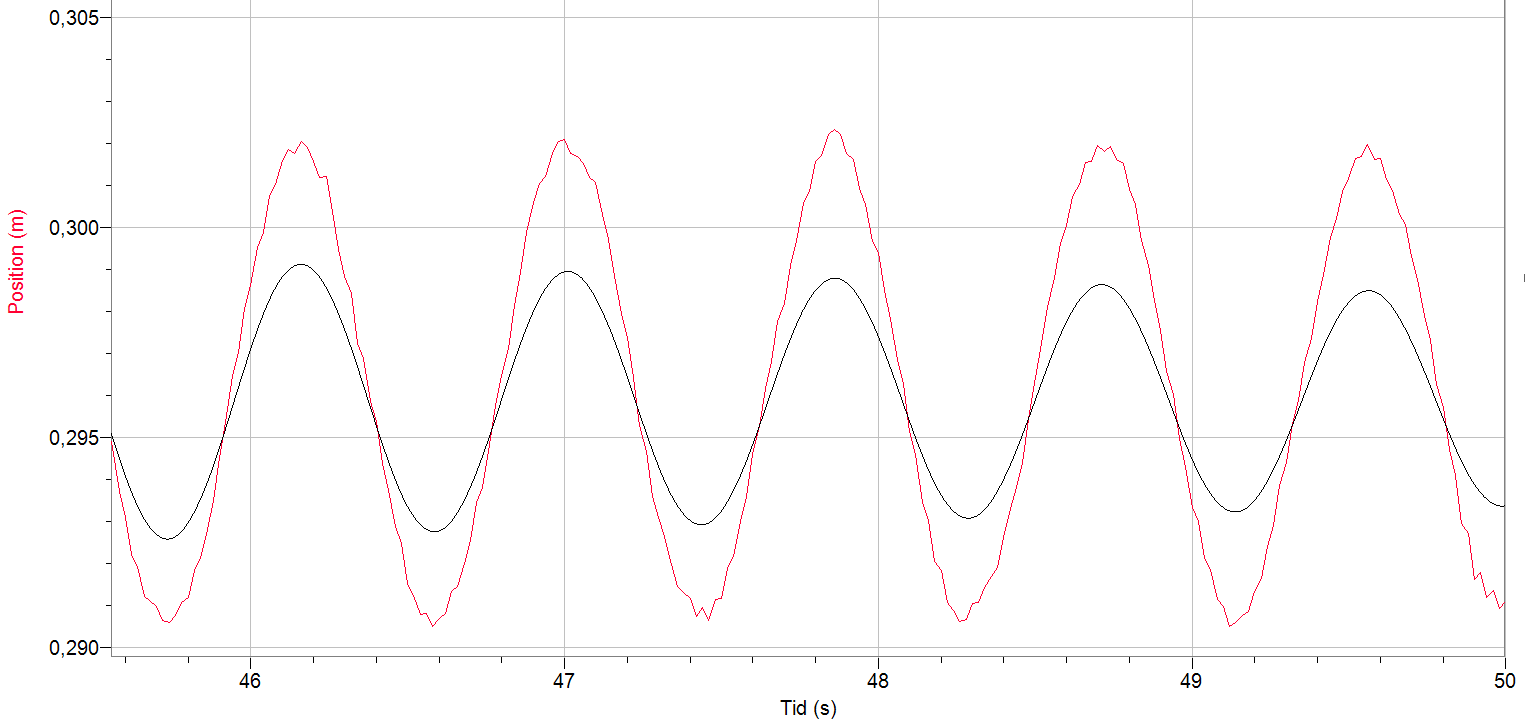
\includegraphics[scale=0.5]{Figurer/Kurvefejl}
\caption{Indzoomet udklik af de sidste ca. $4.5$ sekunder af forsøg E. Det ses her tydeligt at dataen (rød) har et markant større udsving end best-fit-kurven (sort).}
\label{fig: Fejlkurve exp2}
\end{figure}

Grunden til den forskel som ses på figur \ref{fig: Fejlkurve exp2}, er formentlig af vores model for vindmodstanden ikke er helt god nok. 
Med den teori vi har om vindmodstand fra afsnit \ref{teori:vindmodstand}, vil det være et logisk gæt at sige at vi skal have en anden eksponent på vindmodstanden end 1. 

Da teorien siger at vi bør have en eksponent på 2, kan denne forskel måske tilskrives at modellen ikke har den rigtige eksponent.
Vi kan dog ikke, som vi så i afsnit \ref{teori: Den ikke-linear andenordens ligning}, kan vi ikke finde en symbolsk løsning til ligningen med eksponent 2, og vi kan derfor ikke lave et curve-fit. 
Vi kan dog godt lave numeriske løsninger for de to modeller hvor deres koefficienter er de samme, og så observere om modellen med potens på opfører sig på samme måde i forhold til den lineære model som mit data gør i forhold til den lineære model.

Den lineære model vi vil kigge på vil klart nok være på nedenstående form, da det er denne vi har kigget på hele vejen igennem:

\begin{equation}
mx'' + \mu x' + kx = 0
\label{eq: standard linear diff}
\end{equation}
 

Før vi kan opsætte en den ikke-lineære differentialligningsmodel, er vi nødt til at tackle det problem der opstår i at vi mister fortegnet på $x'$ i det at vi sætter det i anden.
Dette problem kan vi løse med at gange størrelsen $\frac{x'}{|x'|}$ på leddet. 
Denne størrelse har egenskaben at den er positiv hvis $x'$ er positiv og negativ hvis $x'$ er negativ. 
Det eneste problem det skaber er at størrelsen er udefineret når $x'=0$, men dette er ikke et stort problem når man laver numeriske løsninger, da man med meget lille sandsynlighed vil ramme netop 0, men oftere nogle meget lange kommatal. 

Vi kan nu opsætte den ikke-lineære differentialligning, hvor $x'$ er sat i anden potens:

\begin{equation}
mx'' + \frac{x'}{|x'|} \mu  (x')^2 + kx = 0
\label{eq: diff i anden}
\end{equation}

Derudover skal vi bruge nogle startværdier for $x$ og $x'$ for at kunne lave en numerisk løsning.
Vi kan tænke os frem til en startværdi for $x'$, da loddet ikke har en fart inden vi giver slip på loddet. 
Startværdien af $x$ svarer til den mængde vi har hevet loddet ud fra sin udgangsposition. 
Da vi kun vil undersøge hvordan de to kurver forholder sig til hinanden, er det ikke så vigtigt hvad vi starter med, og jeg sætter derfor bare værdien til $10$.

For at kunne lave den numeriske løsning, skal vi nu bare have nogle værdier af $m,k$ og $\mu$. 
Jeg vælger disse så de minder om det jeg har fundet i min databehandling. 
På figur \ref{fig: numeriske solutions} kan man se de numeriske løsninger. 

\begin{figure}[h]
\centering
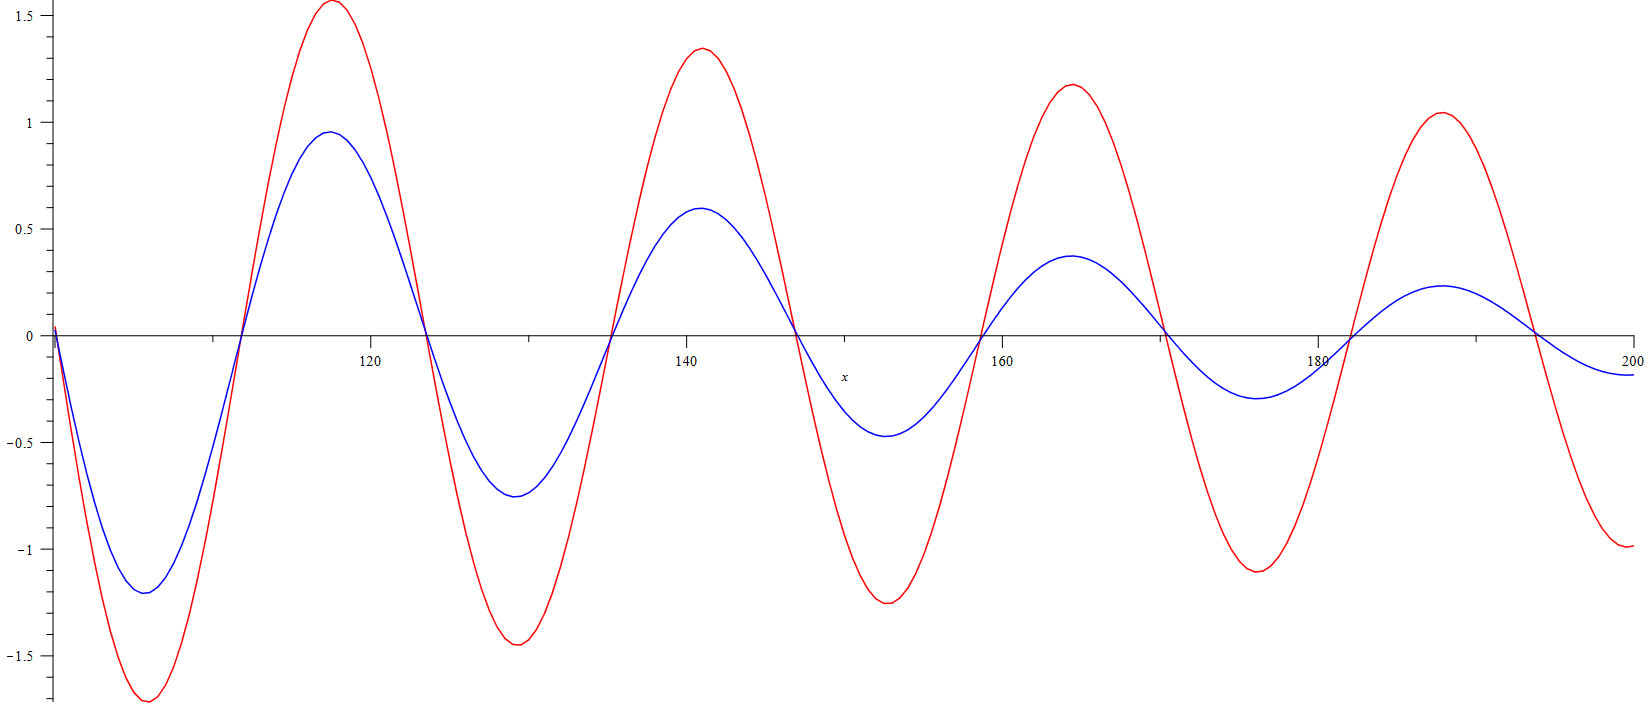
\includegraphics[scale=0.45]{Figurer/diffligninger}
\caption{Sammenligning af numeriske løsninger for differentialligninger \ref{eq: standard linear diff}(blå) og \ref{eq: diff i anden}(rød) et stykke henne ad 1.-aksen, med $m=50,k=3.6,\mu=2$}
\label{fig: numeriske solutions}

\end{figure}

Hvis vi nu betragter figur \ref{fig: Fejlkurve exp2} med figur \ref{fig: numeriske solutions}, så ser vi at de er meget ens. 
Den blå kurve der har det mindste udsving ligner selvfølgelig best-fit-kurven på figur \ref{fig: Fejlkurve exp2}, da de er dannet fra den samme differentialligning. 
Det der er interessant, er at den røde kurve forholder sig på den samme måde til den blå på figur \ref{fig: numeriske solutions}, som mit data forholder sig til best-fit-kurven på figur \ref{fig: Fejlkurve exp2}. 
Dette tyder nemlig på at den ikke-lineære model ville have kunnet beskrive mit datasæt bedre. 





\subsection{Konklusion}
Den lineære homogene andenordens differentialligning er en forholdsvist god model til at beskrive bevægelsen, men den er ikke perfekt. 
Den kurve der produceres fra differentialligningen har træk der minder meget om den rigtige kurve, men jo længere tid der går, jo dårligere viser det sig at den beskriver bevægelsen. 
Det viser sig også at ikke-lineær differentialligningsmodel hvor dæmpningsledet er i anden, beskriver bevægelsen bedre, specielt når vi kigger på svingninger i længere tid.

